% !TEX root = ../main.tex
% Chapter 1

-- Overall todo's --
\begin{itemize}
  \item \TODO{The term \emph{emperical data/distruction} is nowhere used in the thesis. or: Emperical cumulative distribution. Especially Chapter 2.}
  \item \TODO{Check for ``tang-constructions'': saying to much in a single sentence.}
  \item \TODO{Overall: meer focus op de \emph{waarom} vraag/antwoord bij keuzes. Bouwt aan motivatie en context van het geheel.}
  \item \TODO{Consistent `data point' of `data object' gebruiken.}
\end{itemize}

\chapter{Introduction}

\label{Chapter1} % For referencing the chapter elsewhere, use~\ref{Chapter1}

\lhead{Chapter 1. \emph{Introduction}} % This is for the header on each page - perhaps a shortened title

With the wide availability of smartphones and built-in inertial sensors, more and more applications of \gls{har} are introduced \cite{avci2010activity,derawi2010accelerometer,guenterberg2009distributed}.
Many approaches to recognize the performed activity rely on classification of recorded data \cite{devaul2001real,ward2006activity,yang2008using,anguita2012human,bao2004activity,bernecker2012activity,he2008activity}, which can be done online or in batches after the performance \cite{duque2012offline}.
Often a time-windowed based approach is used, which feeds short consecutive segments of data through a model construction and recognition phase.
The constructed model is used to determine which (earlier learned) activity is performed.
Besides the explicit classification of the data, an implicit obtained result is a segmentation of performed activities over time.

In this thesis the goal is to find the temporal segmentation of time series data explicitly, prior to the classification of the activities.
This is done under the assumption that it could be beneficial for classification methods to possess this explicit segmentation, since the model construction phase can use more data than the time-windowed approach would allow.
To find a temporal segmentation, we rely on change detection in time series data.
In the context of this research, this time series data consists of recordings from inertial sensors found in smartphones, such as the accelerometer signal, during the performance of human activities.
We are interested in both in- and outdoor activities in an uncontrolled environment and in a continuous manner, which can be regarded as real-world data.
Although the number of performed activities will be limited, we assume the temporal segmentation must be more robust then in the case of data from a controlled environment.

For the change detection algorithm we have used a special form of \gls{svm}, the \gls{occ} based \gls{svdd} as introduced by Tax~\cite{tax2001one}.
This method models the data under consideration in the shape of a high-dimensional hypersphere.
From this hypersphere the radius is extracted, which can be used as an indication of change and be processed by one-dimensional change detection algorithms.
Since a change in data characteristics, resulting from a change in performed activity, alters the data distribution, the model and thus the radius should reflect this change as well.

\section{Scope}
The scope of this thesis is to find a temporal segmentation of time series data from inertial sensors embedded in smartphones, obtained during the performance of human activities.
As mentioned above, the segmentation is often obtained as a by-product from direct windowed classification.
Other approaches have a very rigid form of segmentation, \eg by limiting the number of possible segment types \cite{himberg2001time,chamroukhi2013joint}, or have applied it to different type of time series data \cite{li2007segmentation,fuchs2010online,guenterberg2009automatic}.
Others have extracted features from windows of data which are used for the segmentation \cite{guo2012adaptive}.
These activities include sitting, standing, walking, running, and ascending and descending staircases.
The problem of finding a temporal segmentation can be seen as a sub-problem to the problem of Activity Classification.
This relation is illustrated in \Cref{fig:thesis_goal}.
The figure shows that we can apply classification over windows of the time series data.
In many approaches this is constructed with a (partially overlapping) sliding window.
In the context of \gls{har}, the window length commonly consists of around $2$ seconds of data points.
In our setup, we create a temporal segmentation instead of a fixed window length.
Each segment should consist of homogeneous data, in the sense that the underlying data generating activity should not change within a segment.
Likewise, the previous and next segments (if present) should be generated by a different performed activity.

To find these segments of homogeneous data, we employ a model construction phase.
The \gls{oc-svm} model transforms the data points to a high-dimensional hyperspherical shape from which we extract the radius as characterizing metric.
In this phase the data is processed by a fixed window length and a change in data characteristics should reflect in a (significant) change of the hypersphere's radius.
Such a sudden change in the radius thus indicates a change in the time series data and indicates the end of the current and beginning of a new segment.
In \Cref{sec:literature_review_temporal_segmentation} a more detailed overview of temporal segmentation methods is discussed.
The information about segments can be used in the classification phase of \gls{har}, which applies classification to windows (or in this case: segments) of data.
The final result, which is outside the scope is this thesis, will be a full classification of activities over the time series data.

\begin{figure}
  \centering
    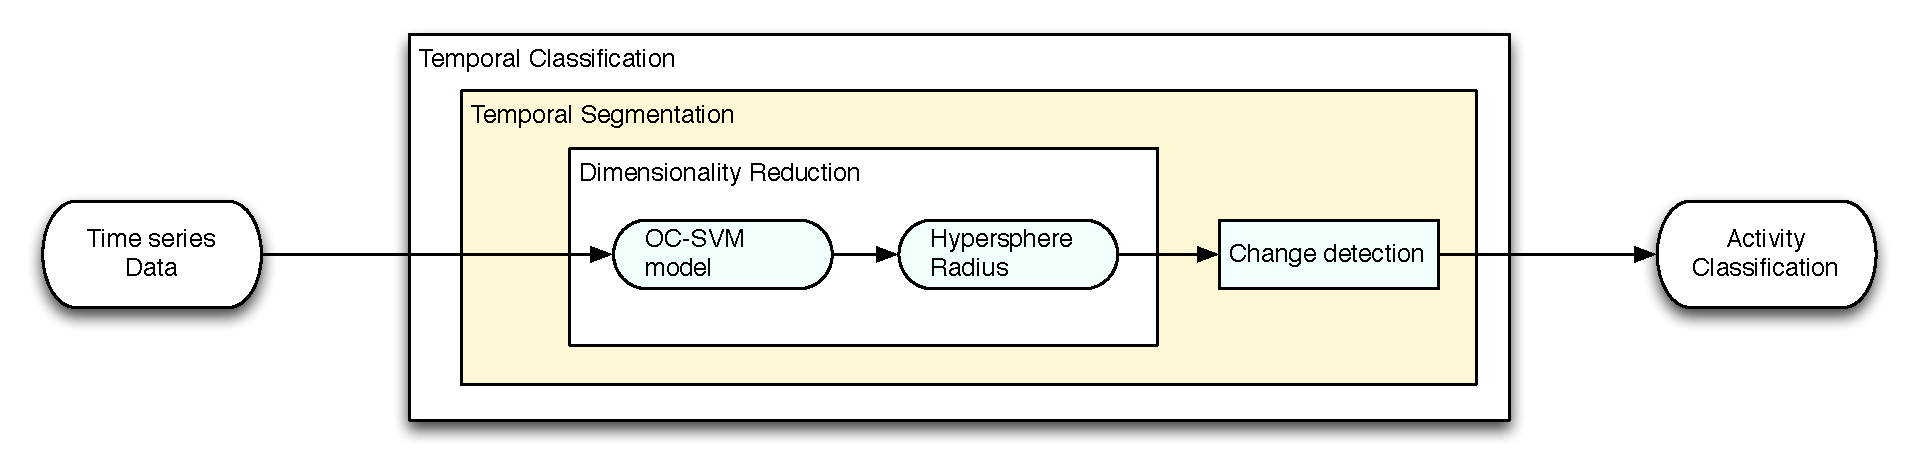
\includegraphics[width=\textwidth,height=\textheight,keepaspectratio]{./Figures/chapter1/thesis_goal.pdf}
  \caption[Thesis goal]{The goal of this thesis. The scope of this thesis is Temporal Segmentation, which can be useful in the context of Temporal Classification. Given a data set, we construct a \gls{oc-svm} high-dimensional spherical model, from which we extract the radius. This metric is then applied to direct change detection algorithms. The detected change points can support the classification of homogeneous segments of data.}
  \label{fig:thesis_goal}
\end{figure}

\section{One-Class Support Vector Machines}
In the setup, as described in the previous section, we employ a model construction phase.
For this model we will use an \acrlong{oc-svm} implementation: the \acrlong{svdd} algorithm by Tax~\cite{tax2001one}.
In earlier research multi-class \glspl{svm} are used for direct classification of inertial sensor data \cite{he2008activity,mountrakis2011support,anguita2012human}.
Others have used \gls{oc-svm} classifiers for novelty, or outlier, detection \cite{scholkopf1999support,camci2010change,li2003improving,ma2003time,tax1999support}.
The research by Yin \etal  \cite{yin2008sensor} creates a \gls{oc-svm} classifier to filter normal activity traces, using training data.
However, to the best of our knowledge, \gls{oc-svm} methods have not yet been applied to inertial sensor time series data directly to find changes in behavior and create a temporal segmentation.
This algorithm transforms the time series data, which can be of any high dimension, to an higher dimensional feature space.
When the data is assumed to be of the same class, it can be characterized by an enclosing boundary, in the shape of a hypersphere.
Using this \gls{occ} method, we are able to test new data points of being a member of this class.
When a new data point, after transformation to the feature space, lies within the boundary, it is a member of the class, and otherwise it is regarded as an outlier.

In case the data distribution changes, the data points will have a larger variance which results in a larger hypersphere in the feature space.
This means that with continuous model updating, a change in the underlying process of a time series data means the hypersphere will have a larger radius.
Thus the \gls{oc-svm} method allows us to generate a one-dimensional time series data, reduced from a complex high-dimensional original signal.
The final radius time series data can be inspected by simpler change detection methods, in a number of ways.
\Cref{Chapter3} will discuss the \gls{oc-svm} methods in detail and \Cref{Chapter4} elaborates on the overall change detection method.

\section{Data sets}
In recent previous research two data sets for the context of \gls{har} have been made public.
In order to benchmark our proposed method we tried to employ it to these data sets.
However, it turned out the data sets were not appropriate for continuous temporal segmentation.
The first set, the \gls{wisdm} from \cite{kwapisz2011activity}, consists of non-continuous recordings of activities.
Obviously, this voids the usefulness of the data set of our research.
The second set, the \gls{uci-har} from \cite{anguita2012human}, also lacks continuous recordings and furthermore exhibits patterns and labeling which seems to be incorrect.
Besides these problems, since there are no visual images of the performed activities, there is no ground truth which can be consulted in case of ambiguity.
To overcome these problems, we have created our own real-world data sets.

Our own data sets are recorded by placing a smartphone with inertial sensors in the front right pants pocket of a subject.
The subject was asked to perform common and simple activities in an uncontrolled environment, both in- and outdoor situated.
During the performance the subjects were also recorded with a video camera from the third-person point of view.
This allows us to create a ground truth for the temporal segmentation of performed activities.

Besides the recorded data sets we have used artificial data sets to obtain an objective performance measure of the method.
These artificial data sets are modeled to the sets used in \cite{camci2010change,takeuchi2006unifying}.
In \Cref{Chapter5} we discuss the artificial data sets and results in detail.
The real-world recordings and results are discussed in \Cref{Chapter6}.

\section{Contributions}
As a result from our proposed method and application to recorded real-world data sets, this thesis will provide the following contributions:
\begin{enumerate}
  \item \textbf{Continuous recorded human activity data:} the proposed method is applied to our own recorded human activity data.
  This data set can be grounded by using the video recordings of the subject while performing the activities.
  The data set, consisting of raw inertial sensor recordings, manual change point and activity labeling, and video recordings, are used for testing the method and are made publicly available \cite{vlasveld2013continuous}.
  \item \textbf{Application of \gls{oc-svm} methods to inertial sensor data:} to the best of our knowledge, this thesis is the first application of \gls{oc-svm} methods, especially the \gls{svdd} method, to inertial sensor signals in the context of creating a temporal segmentation.
  Furthermore, this thesis contributes to the small amount of research that has a temporal segmentation of inertial sensor data as its primary objective.
  \item \textbf{Adaptation of \acrshort{svcpd}:} we have adopted and slightly adapted the \acrshort{svcpd} method by Camci~\cite{camci2010change} in order to find change points in time series data.
  In our simplification we have not encountered noticeably decrease in performance.
\end{enumerate}

\section{Thesis structure}
The structure of this thesis is as follows.
In \Cref{Chapter2} a literature review is provided.
We will look at the different interpretations and implementations for change, novelty, and outlier detection.
Previous work in the field of \gls{har} is discussed and we end with existing applications of \glspl{svm} to change detection.
The next chapter further analyses \glspl{svm} and two implementations of \glspl{oc-svm}.
It relates the properties of the constructed \gls{oc-svm} models to change detection in time series data.
That relation is applied to our problem formulation in \Cref{Chapter4}, where we construct our change detection method \TODO{add name}, based on the work of Camci~\cite{camci2010change}.
The two following chapters apply the method to both artificial and real-world data.
\Cref{Chapter5} show the objective performance of the method to artificial constructed data.
In \Cref{Chapter6} we apply the method to our self-recorded real-world data.
In that chapter we show the ability of detecting change in \gls{har} data, recorded by inertial sensors.
This thesis is concluded in \Cref{Chapter7}, in which we reflect on the performed research and state possibilities for feature research.